\documentclass[SurvivalMain.tex]{subfiles}
\begin{document}
\Large	
\subsection{AML Data Set}

Acute Myelogenous Leukemia survival data

% Description

\noindent \textbf{Survival in patients with Acute Myelogenous Leukemia. }\\
The question at the time was whether the standard course of chemotherapy should be extended ('maintainance') for additional cycles.

\begin{description}
\item[time:]	survival or censoring time
\item[status:]	censoring status
\item[x:]	maintenance chemotherapy given? (factor)
\end{description}
\begin{verbatim}
> 
> head(aml)
time status          x
1    9      1 Maintained
2   13      1 Maintained
3   13      0 Maintained
4   18      1 Maintained
5   23      1 Maintained
6   28      0 Maintained
> 
\end{verbatim}
%====================================================================================================================
{
	\large
\begin{framed}
\begin{verbatim}
library(survival)
leukemia.surv <- survfit(Surv(time, status) ~ x, 
    data = aml) 

plot(leukemia.surv, lty = 2:3) 
legend(100, .9, 
   c("Maintenance", "No Maintenance"), 
   lty = 2:3) 

title("Kaplan-Meier Curves\nfor AML Maintenance Study") 
\end{verbatim}
\end{framed}
}
\begin{figure}[h!]
\centering
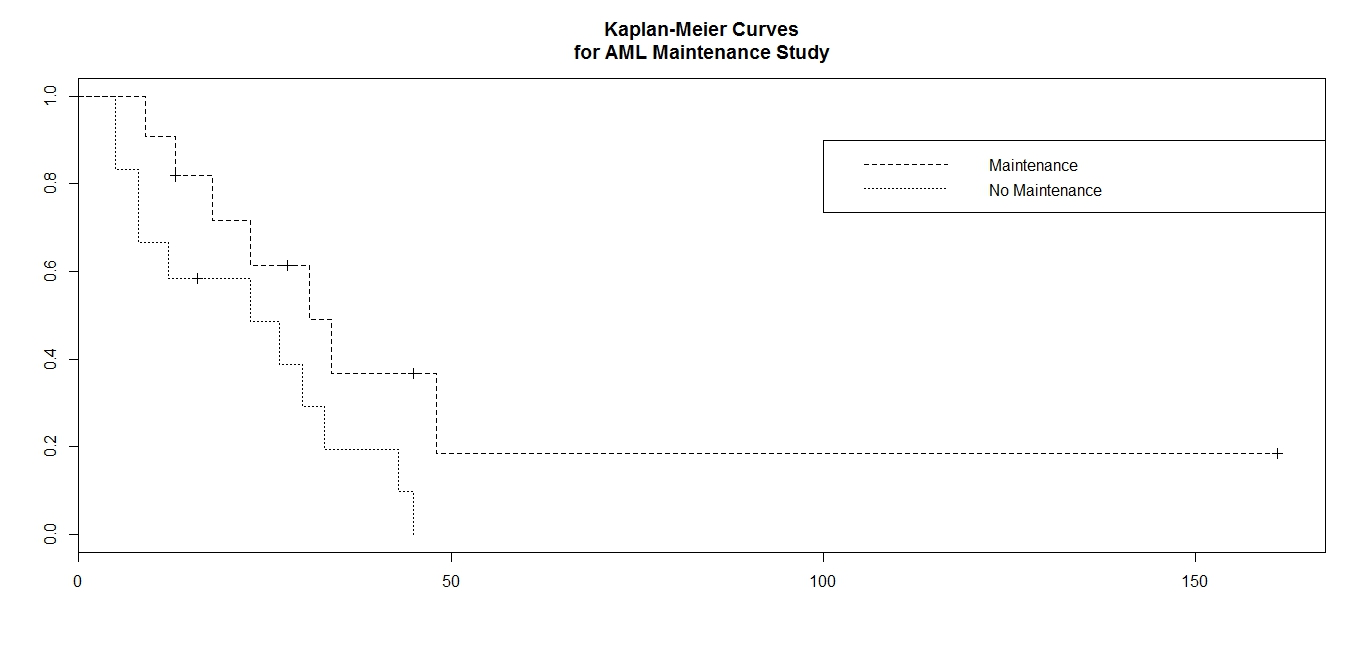
\includegraphics[width=0.7\linewidth]{AML1}
\caption{}
\label{fig:AML1}
\end{figure}



%====================================================================================================================
\begin{framed}
\begin{verbatim}
lsurv2 <- survfit(Surv(time, status) ~ x, aml, type='fleming') 
plot(lsurv2, lty=2:3, fun="cumhaz", 
xlab="Months", ylab="Cumulative Hazard") 
\end{verbatim}
\end{framed}
\begin{figure}[h!]
\centering
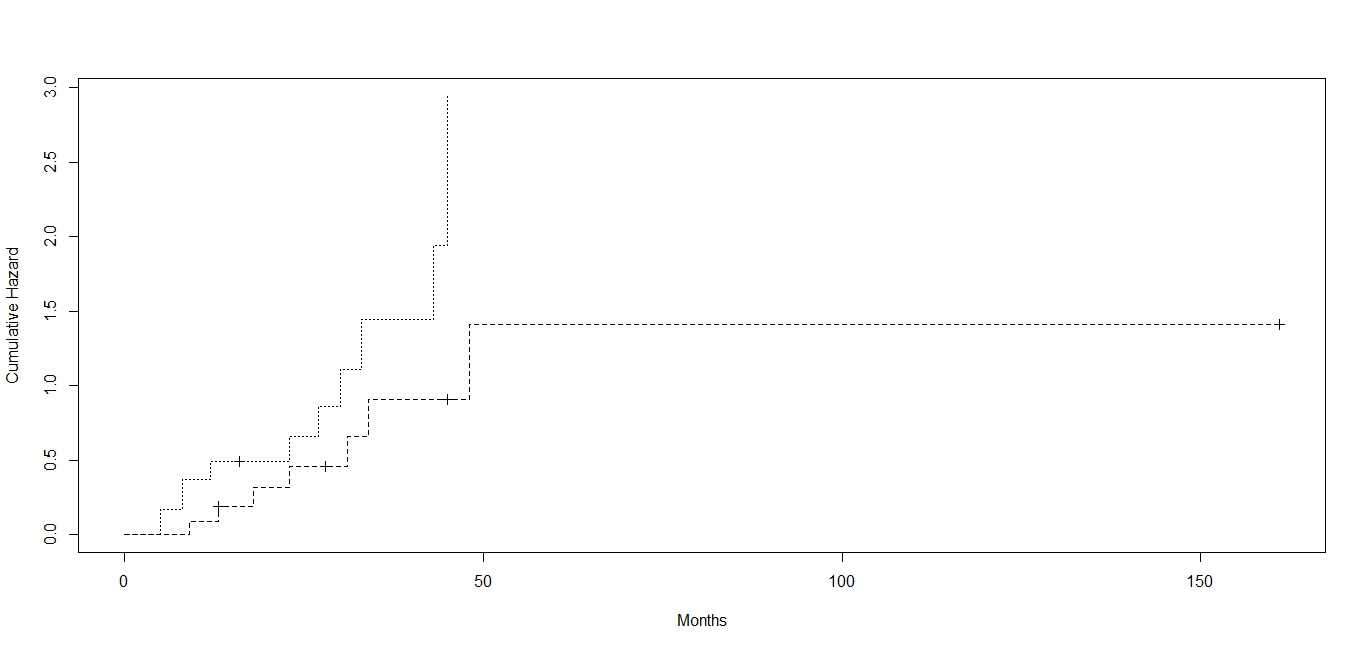
\includegraphics[width=0.7\linewidth]{AML2}
\caption{}
\label{fig:AML2}
\end{figure}

\end{document}
